\documentclass[10pt,twocolumn,letterpaper]{article}

\usepackage{cvpr}
\usepackage{times}
\usepackage{epsfig}
\usepackage{graphicx}
\usepackage{amsmath}
\usepackage{amssymb}
\usepackage{listings}
\usepackage{url}
\usepackage{algorithm}% http://ctan.org/pkg/algorithms
\usepackage{algpseudocode}% http://ctan.org/pkg/algorithmicx
\usepackage{verbatim}
\usepackage{color}
\usepackage{xcolor}
\usepackage[italian]{babel}
\usepackage{caption}
\usepackage{lstcustom}
\usepackage[scaled=0.8]{beramono}
\usepackage[utf8x]{inputenc}
\usepackage{enumitem}
\usepackage{booktabs}

% Include other packages here, before hyperref.

% If you comment hyperref and then uncomment it, you should delete
% egpaper.aux before re-running latex.  (Or just hit 'q' on the first latex
% run, let it finish, and you should be clear).
\usepackage[pagebackref=true,breaklinks=true,letterpaper=true,bookmarks=false]{hyperref}

\cvprfinalcopy % *** Uncomment this line for the final submission


\def\httilde{\mbox{\tt\raisebox{-.5ex}{\symbol{126}}}}

% Pages are numbered in submission mode, and unnumbered in camera-ready
\ifcvprfinal\pagestyle{empty}\fi

\DeclareCaptionFont{white}{\color{white}}
\DeclareCaptionFormat{listing}{\colorbox{gray}{\parbox{\columnwidth}{#1#2#3}}}
\captionsetup[lstlisting]{format=listing,labelfont={white, bf},textfont=white}

\newcommand\myworries[1]{\textbf{\textcolor{red}{#1}}}
\makeatletter
\newcommand{\newalgname}[1]{%
  \renewcommand{\ALG@name}{#1}%
}
\newalgname{Algoritmo}
\renewcommand{\listalgorithmname}{Lista di \ALG@name s}
\renewcommand{\lstlistingname}{Codice}
\renewcommand{\lstlistlistingname}{Lista di codici}
\makeatother

\begin{document}
\lstdefinestyle{customA}{         
	basicstyle=\footnotesize\lstfontfamily,
	emphstyle=\bfseries,
	language=C,
	numberstyle=\tiny,          
	numbersep=5pt,              
	tabsize=2,                  
	extendedchars=true,         
	breaklines=true,            
	keywordstyle=\bfseries\color{green!50!black},
	commentstyle=\itshape\color{purple!40!black},
	frame=b,         
	stringstyle=\color{orange}\ttfamily, 
	showspaces=false,           
	showtabs=false,             
	xleftmargin=1pt, %prima era 17
	framexleftmargin=17pt,
	framexrightmargin=5pt,
	framexbottommargin=4pt,
	showstringspaces=false,     
}
%%%%%%%%% TITLE
\title{PC-2016/17 Progetto mid-term del corso \\
Implementazione in CUDA dell'algoritmo KMean}

\author{Tommaso Ceccarini \\
6242250\\
{\tt\small tommaso.ceccarini1@stud.unifi.it}
% For a paper whose authors are all at the same institution,
% omit the following lines up until the closing ``}''.
% Additional authors and addresses can be added with ``\and'',
% just like the second author.
% To save space, use either the email address or home page, not both
\and
Federico Schipani\\
6185896\\
{\tt\small federico.schipani@stud.unifi.it}
}

\maketitle
\thispagestyle{empty}

%%%%%%%%% ABSTRACT
\begin{abstract}
	L'algoritmo di KMeans è uno dei più popolari metodi per la clusterizzazione. Nel nostro lavoro forniamo una implementazione in CUDA che fa uso 
	di GPU Nvidia per l'esecuzione dell'algoritmo. Inoltre forniamo un'analisi delle preformance con lo scopo di comparare la nostra implementazione parallela con una implementazione sequenziale scritta in C.
\end{abstract}

%%%%%%%%% BODY TEXT
\section{Introduzione}
L'algoritmo KMeans è uno degli algoritmi di clustering più famosi. Lo scopo del clustering è di dividere dati in gruppi significativi chiamati cluster.
Dato un insieme di dati $(\boldsymbol{x_{1}}, \boldsymbol{x_{2}}, \dots,\boldsymbol{x_{N}} )$ dove ogni dato è un vettore reale di dimensione $P$, lo scopo di KMeans è di partizionare $N$ dati in $K (\leq N)$ insiemi $\boldsymbol{S} = \{S_{1}, S_{2}, \dots, S_{K}\}$ per minimizzare la distanza dentro ai singoli cluster. In altre parole viene definita una funzione obiettivo del tipo: 
\begin{equation}
\label{eq:first}
\operatorname*{arg\, min}_{\boldsymbol{S}} \displaystyle\sum_{i = 1}^{k} \displaystyle\sum_{x \in S_{i}} ||\boldsymbol{x} - \boldsymbol{\mu}_{i} ||^{2}
\end{equation}  
dove $\mu_i$ è la media dei punti in $S_{i}$.\cite{wiki:kmeans}
\par
\begin{algorithm}
\caption{KMeans}
\label{alg:kmeans}
\begin{algorithmic}[1]
\Procedure{KMeans}{$\text{data}[\text{n}][\text{p}]$}
\State $\text{mean}[\text{k}][\text{p}], \text{oldMean}[\text{k}][\text{p}]$
\State $\text{assignment}[\text{n}]$
\State $(\text{mean}, \text{assignment}) \leftarrow initAss(data)$
\While{$!stop$}
\State $\text{assignment} \leftarrow calcMin(\text{mean}, \text{data})$
\State $\text{oldMean} \leftarrow \text{mean}$
\State $\text{mean} \leftarrow calcMean(\text{assignment}, \text{data})$
\State $\text{stop} \leftarrow stopCrit(\text{mean}, \text{oldMean})$
\EndWhile
\State \textbf{return} $\text{mean}$
\EndProcedure
\end{algorithmic}
\end{algorithm}
L'Algoritmo \ref{alg:kmeans} rappresenta lo pseudocodice di un'implementazione iterativa dell'algoritmo KMeans.

I principali passi dell'algoritmo sono:
\begin{enumerate}
	\item{Selezionare casualmente K dati per inizializzare la media dei K cluster. Questo passo è usualmente chiamato \textit{inizializzazione}.}
	\item{Assegnare ogni dato al cluster più vicino, in accordo ad certa funzione di distanza. Questo passo è chiamato \textit{assegnamento}.}
	\item{Calcolare la nuova media dei cluster. Questo passo è chiamato \textit{aggiornamento}.}
	\item{Ripetere il passo due e tre finché nessun dato cambia cluster, oppure se solo pochi lo fanno.}
\end{enumerate}
\subsection{KMeans sequenziale}

Prima del ciclo \textit{while} c'è un passo di assegnazione iniziale. In questo step i primi $K$ dati sono assegnati ai primi $K$ cluster. Uno pseudocdice di questo assegnamento iniziale è mostrato in Algoritmo \ref{alg:initialAssignment}
\begin{algorithm}
\caption{Initial Assignment}
\label{alg:initialAssignment}
\begin{algorithmic}[1]
\Procedure{initAss}{$\text{data}[\text{n}][\text{p}]$}
\State $\text{mean}[\text{k}][\text{p}]$
\State $\text{assignment}[\text{n}]$
\For{$\text{i} = 0; \text{i}<\text{k}; \text{i}++$}
\State $\text{assignment}[\text{i}] = \text{i}$
\For{$\text{j} = 0; \text{j} < \text{p}: \text{j}++$} 
\State $\text{mean}[\text{i}][\text{j}] = \text{data}[\text{i}][\text{j}]$
\EndFor
\EndFor
\State \textbf{return} $\text{(mean, assignment)}$
\EndProcedure
\end{algorithmic}
\end{algorithm}

Dopo questo step iniziale di assegnamento parte il vero e proprio algoritmo. Nella prima parte del ciclo \textit{while} viene calcolata la distanza euclidea minima tra ognuno dei dati e tutti i cluster. Successivamente si assegna ogni dato al cluster più vicino.
Il passo successivo consiste nel ricalcolare le nuove medie dei cluster, secondo la \eqref{eq:mean}. 
\begin{equation}
\label{eq:mean}
m_i^{(t+1)} = \frac{1}{|S^{(t)}_i|} \displaystyle\sum_{x_{j} \in S^{(t)}_i} x_j 
\end{equation}


L'ultimo step è il criterio d'arresto. In questo semplice algoritmo, mostrato in \ref{alg:stopCriterion}, si iterano l'attuale matrice dei cluster e la matrice dei cluster calcolata al passo $i-1$. Quando $ActualValue - OldValue$ eccede una prefissata tolleranza TOL  il metodo ritorna il valore \textit{false}. Questo valore di ritorno porterà ad un'altra iterazione del ciclo \textit{while} esterno.

\begin{algorithm}
\caption{Stop Criterion}
\label{alg:stopCriterion}
\begin{algorithmic}[1]
\Procedure{stopCrit}{$\text{mean}[\text{k}][\text{p}], \text{oldMean}[\text{k}][\text{p}]$}
\ForAll{value, oldValue in  mean, oldMean}
\If{$abs(value - oldValue) > \text{TOL}$}
\State \textbf{return} false
\EndIf
\EndFor
\State \textbf{return} true
\EndProcedure
\end{algorithmic}
\end{algorithm}


\section{Implementazione}
\subsection{Come vengono rappresentati i dati ed i cluster}
Le due differenti implementazioni dell'algoritmo di KMeans, riportate in sezione  ~\ref{sub:Cimpl} e ~\ref{sub:cudaimpl}, risolvono il problema del clustering per  un valore arbitrario del parametro $P$. Tuttavia le analisi delle performance, mostrate in Sezione~\ref{sec:performanceanalysis}, sono state effettuate nel caso in cui $P=2$, ovvero il caso in cui i dati sono vettori bidimensionali. \par
Le due maggiori strutture su cui il codice lavora sono la matrice dei dati e la matrice dei centroidi, rispettivamente di dimensione $N*P$ e $K*P$. In entrambe le implementazione viene usato anche un vettore chiamato \textit{assignment} che, per tutti gli $N$ dati, memorizza l'indice del cluster al quale appartengono.

\subsubsection{Come viene generato il dataset}
Dopo che sono state dichiarate, e successivamente istanziate, le strutture che sono necessarie per rappresentare i dati e i centroidi viene effettuata una genrazione pseudocasuale dei dati. Questa generazione viene effettuata in maniera parallela attraverso le API CUDA, in particolare è stata usata la libreria cuRAND. Il metodo che è stato sviluppato per questo scopo è \texttt{generateRandomDataOnDevice()}. Questo metodo usa un seed prefissato e, con l'aiuto di un altro metodo che fa parte della libreria cuRAND, genera i valori del dataset. Nella Sezione~\ref{sec:performanceanalysis} sono mostrate le analisi delle performance nel caso in cui i dati sono generati con una distribuzione uniforme. 

\subsection{Una implementazione sequenziale in C}

\label{sub:Cimpl}

\subsubsection*{Lo step di inizializzazione}
Dopo aver generato casualmente il dataset nella memoria globale del device è necessario istanziare la memoria richiesta per memorizzare la matrice dei dati e dei centrodi nella memoria dell'host. Inoltre, per come funziona l'algoritmo, è necessaria un'altra matrice che memorizza il valore della media durante la precedente iterazione. Questa matrice è usata per implementare il criterio d'arresto. L'inizializzazione è effettuata da un semplice ciclo for che assegna \texttt{data[i][j]} a \texttt{mean[i][j]} per  \texttt{i} tra $0$ e $K-1$. Questa strategia d'assegnamento è motivata dal fatto che i dati sono generati casualmente.
\subsubsection*{Lo step di assegnamento}
Dopo aver effettuato l'assegnazione iniziale l'algoritmo sequenziale implementa il passo di assegnamento attraverso il Codice~\ref{code:assseqe}. Nel Codice~\ref{code:assseqe} vengono utilizzati due cicli for: un ciclo esterno che itera su $N$ dati e un ciclo annidato che per ogni dato itera sui $K$ cluster per cercare il più vicino. Al termine del ciclo annidato l'indice del cluster più vicino al dato \texttt{i}-esimo verrà memorizzato alla cella \texttt{i} del vettore \texttt{assignment[]}.
\lstinputlisting[firstline = 17, lastline = 34, caption = Passo di assegnamento sequenziale, style = customA, label = {code:assseqe}]{Codice/sequential.c}
\subsubsection*{Lo step di aggiornamento}
Successivamente all'assegnazione dei dati al cluster più vicino è necessario ricalcolare nuovamente i valori dei centroidi per i cluster. Questo passo dell'algoritmo è implementato mediante il Codice~\ref{code:aggmedia}. Come si può notare dal Codice~\ref{code:aggmedia} questo passo è implementato mediante due cicli for: un primo ciclo esterno che itera sui $K$ cluster e un ciclo annidato in cui, utilizzando il vettore \texttt{assignment[]} viene calcolata la somma dei valori delle singole componenti dei dati che appartengono al cluster e il numero di dati che appartengono al cluster. Quindi alla fine del ciclo interno, per ogni componente, viene diviso il valore della somma per il numero di dati che appartengono al cluster per calcolare il valore effettivo dei nuovi centroidi.
\lstinputlisting[firstline = 35, lastline = 53, caption = Passo di aggiornamento della media, style = customA, label = {code:aggmedia}]{Codice/sequential.c}
\subsubsection*{Il criterio d'arresto}

Il criterio d'arresto che viene implementato verifica se il vettore dei centroidi è cambiato nel corso dell'ultima iterazione rispetto a una prefissata tolleranza \texttt{TOL}. Per implementare questa strategia, alla riga 16 del Codice~\ref{code:aggmedia}, prima di aggiornare il valore della media, vengono copiati i valori di \texttt{mean[]} nel vettore di appoggio \texttt{oldMean[]}. Il Codice~\ref{code:stopcritseq} verifica quindi se i valori dei centroidi sono cambiati iterando mediante un ciclo for sulle componenti dei vettori \texttt{oldMean[]} e \texttt{mean[]} verificando se i valori sono uguali a meno di una tolleranza \texttt{TOL}.

\lstinputlisting[firstline = 54, lastline = 60, caption = Criterio di arresto sequenziale, style = customA, label = {code:stopcritseq}]{Codice/sequential.c}
\subsection{Implementazione parallela tramite CUDA}
\label{sub:cudaimpl}
\subsubsection{Benefici di un'implementazione parallela}
\label{sec:benefici}
In riferimento al codice sequenziale si può notare come gran parte dei calcoli che vengono effettuati siano indipendenti gli uni dagli altri. Questo fatto porta a pensare che un'implementazione parallela avrà dei miglioramenti in termini di prestazioni. In particolare le operazioni parallelizzabili sono:
\begin{itemize}
	\item{Assegnazione iniziale. Infatti è possibile assegnare ad un thread il compito di assegnare il valore di una componente del centroide.}
	\item{Calcolo delle distanze. Ciascuna delle $N*K$ distanze può essere calcolata indipendentemente dalle altre.}
	\item{Determinazione del cluster più vicino. In questo contesto è possibile assegnare ad un thread il compito di determinare quale sia il cluster più vicino ad un dato. In ogni caso è comunque necessario effettuare una ricerca sequenziale scorrendo $K$ medie.}
	\item{Calcolo della media. Utilizzando il vettore degli assegnamenti ogni thread può: determinare a quale cluster il dato corrispondete appartiene, e incrementare il contatore del numero di elementi per cluster che servirà poi per il calcolo effettivo della media. }
\end{itemize}
Seguendo queste idee quindi è stato implementato il metodo \texttt{kMeans(float *devData, short* devAssignment, float* devMean)} che riceve in input la matrice dei dati, il vettore degli assegnamenti e la matrice dei centrodi, tutte queste strutture sono allocate nella memoria del device.
\subsubsection*{Lo step di inizializzazione}
Per realizzare il passo di inizializzazione vengono utilizzati i due metodi Kernel riportati in Codice~\ref{code:initass} e Codice~\ref{code:initmean}.
\lstinputlisting[firstline = 52, lastline = 57, caption = Assegnazione iniziale dei dati ai cluster, style = customA, label = {code:initass}]{Codice/KMeans.cu}
Nel Codice \ref{code:initass} viene effettata l'assegnazione iniziale. Questo viene eseguito con un totale di $K$ thread. Ogni thread che esegue questa funzione Kernel si occupa di inizializzare il vettore degli assegnamenti scrivendo in posizione \texttt{index} il proprio indice \texttt{index}. A questo scopo la dimensione dei blocchi viene impostata a \texttt{dim3 DimBlockInizPart(1024, 1, 1)} e di conseguenza la griglia sarà inizializzata a \texttt{dim3 DimGridInizPart((k / 1024) + 1, 1, 1)}.
\lstinputlisting[firstline = 58, lastline = 71, caption = Inizializzazione della matrice dei centroidi, style = customA, label = {code:initmean}]{Codice/KMeans.cu}
Dopo aver assegnato i primi $K$ dati ai relativi cluster il Codice \ref{code:initmean} si occupa di assegnare sfruttando questo fatto: infatti è sufficiente assegnare i valori delle componenti del dato \texttt{(i, j)} al centroide \texttt{(i, j)}. Quindi in questo caso vengono usati $K*P$ thread e la dimensione dei blocchi viene impostata a \texttt{dim3 DimBlockInizMean(P, 16, 1)}, e di conseguenza la griglia sarà inizializzata a \texttt{dim3 DimGridInizMean(1, k / 16 + 1, 1)}.
\subsubsection*{Lo step di assegnamento}
Per parallelizzare il passo di assegnamento vengono usate due funzioni, riportati in Codice~\ref{code:comptdist} e Codice~\ref{code:compmin}.
L'implementazione parallela del passo di assegnamento è realizzata attraverso i due metodi riportati in Codice~\ref{code:comptdist} e Codice~\ref{code:compmin}. Nel Codice~\ref{code:comptdist} ogni thread \texttt{(i,j)} è responsabile del calcolo della distanza del dato \texttt{i} dal cluster \texttt{j}. Quindi la griglia dei blocchi è organizzata in \texttt{dim3 DimGridDistances((k / 4) + 1, (n / 256) + 1, 1)} e di conseguenza i blocchi sono stati impostati a \texttt{dim3 DimBlockDistances(4, 256, 1)}.\par

\lstinputlisting[firstline = 130, lastline = 148, caption = Kernel per il calcolo delle distanze, style = customA, label = {code:comptdist}]{Codice/KMeans.cu}
L'altro Kernel riportato nel Codice~\ref{code:compmin} effettua la ricerca del cluster più vicino al dato utilizzando la matrice delle distanze appena calcolata dal Codice~\ref{code:comptdist}. In questo contesto vengono utilizzati $N$ thread in cui ciascuno effettua una ricerca sequenziale della distanza minima, memorizzando allo stesso tempo l'indice del cluster più vicino. La griglia è organizzata come \texttt{dim3 DimGridMin(1, (n / 256) + 1, 1)}, e i blocchi come \texttt{dim3 DimBlockAss(1, 256, 1)}.\par

\lstinputlisting[firstline = 150, lastline = 165, caption = Kernel per il calcolo del minimo, style = customA, label = {code:compmin}]{Codice/KMeans.cu}


\subsubsection*{Lo step di aggiornamento}

L'aggiornamento della media è divisa in tre Kernel, riportati in Codice~\ref{code:initvector}, Codice~\ref{code:sum37} e Codice~\ref{code:mean37}.
Il metodo Kernel, riportato in Codice~\ref{code:initvector}, si occupa di reinizializzare il valore dei centroidi a 0. Questo per realizzare il calcolo delle somme delle componenti dei dati in modo atomico, riportato nel Codice~\ref{code:sum37}. 

\lstinputlisting[firstline = 42, lastline = 50, caption = Kernel per reinizializzare un vettore, style = customA, label = {code:initvector}]{Codice/KMeans.cu}
Il Codice~\ref{code:sum37} utilizza $N*P$ thread in cui il thread \texttt{(i,j)} si occupa di verificare, attraverso il vettore degli assegnamenti a quale cluster appartiene la componente \texttt{j} del dato \texttt{i} e di incrementare il conteggio degli elementi appartenenti al cluster del dato.

\lstinputlisting[firstline = 73, lastline = 90, caption = Calcolo della somma e del numero di elementi di un cluster, style = customA, label = {code:sum37}]{Codice/KMeans.cu}

Infine nel Codice~\ref{code:mean37}, $K*P$ thread si occupano di fare il calcolo effettivo della media dividendo il risultato delle somme calcolate nel Codice \ref{code:sum37} per il numero di elementi che appartengono al relativo cluster. I $K*P$ thread sono divisi in blocchi \texttt{dim3 DimBlockMean(P, 256, 1)} e la griglia è formata da \texttt{dim3 DimGridMean(1, (K / 256) + 1, 1)} blocchi.
\lstinputlisting[firstline = 92, lastline = 106, caption = Kernel per il calcolo della media, style = customA, label = {code:mean37}]{Codice/KMeans.cu}
\subsubsection*{Il criterio d'arresto}

Per implementare il criterio d'arresto sono state prese in considerazione due possibili strade:
\begin{enumerate}
	\item\label{enum:seq1} Utilizzare una variabile globale che conta il numero di dati che cambiano il cluster di appartenenza nel corso di una singola iterazione.
	\item\label{enum:seq2} Riutilizzare il criterio di arresto implementato per la versione sequenziale, mostrato in Codice \ref{code:stopcritseq}
\end{enumerate}
L'implementazione della possibilità \ref{enum:seq1} è stata realizzata incrementando atomicamente la variable globale in questione tutte le volte in cui il Codice \ref{code:compmin} determina un cambiamento di cluster. Questa soluzione porta ad un incremento della divergenza a causa del controllo necessario per verificare se il cluster del dato cambia. Quindi è stata valutata la possibilità di riutilizzare il codice che effettuava il criterio d'arresto nell'implementazione dell'algoritmo sequenziale. Sono state condotte una serie di verifiche per determinare se ci fossero delle differenze in termini di prestazioni tra le due diverse possibilità. A seguito di queste verifiche è stato riscontrato che la versione sequenziale del criterio d'arresto è generalmente, anche se di poco, migliore della controparte parallela.\par
Per realizzare una versione più efficiente della possibilità \ref{enum:seq2} è stata considerata la possibilità di effettuare una verifica parallela sul vettore delle medie utilizzando la tecnica di riduzione. Ad ogni modo verifiche condotte in merito hanno mostrato che tale approccio non portava alcun tipo di beneficio in termini di prestazioni. Questo tipo di tecnica ha il merito di sfruttare al meglio le potenzialità della memoria shared utilizzandole in maniera efficiente, e senza generare conflitti, per ridurre un vettore ad un singolo elemento. D'alta parte questo approccio richiede di iterare sempre e comunque su tutto il vettore per decidere il risultato finale del controllo, mentre la versione sequenziale appena verifica che una media nel corso dell'ultima iterazione è cambiata a meno di una tolleranza \texttt{TOL} si ferma restituendo il fallimento del controllo. Ad ogni modo dovendo operare su strutture allocate nella memoria del host sono necessarie due \texttt{cudaMemCpy()} del tipo \texttt{DeviceToHost} per il vettore delle medie aggiornato e quello vecchio.
\section{Analisi delle performance e risultati sperimentali}
\label{sec:performanceanalysis}



Una volta che le due diverse versioni dell'algoritmo di KMeans sono state sviluppate sono stati condotti una serie di esperimenti per verificare quale fosse il vantaggio effettivo ottenuto dall'implementazione parallela.
Le Figure ~\ref{fig:test} ~\ref{fig:test2} ~\ref{fig:test3} riportano il risultato della clusterizzazione ottenuta attraverso l'implementazione in CUDA con diversi valori di $N$ e $K$.
\subsection{Tempi di esecuzione}
In Tabella~\ref{my-label} sono riportati i tempi di esecuzione per i due algoritmi implementati. Come si può osservare consultando la tabella la versione parallela è migliore di quella sequenziale. I risultati riportati sono stati ottenuti impostando un valore della tolleranza di  $5 * 10^{-6}$. In Tabella~\ref{speedup} è riportato lo speedup che la versione parallela raggiunge rispetto a quella sequenziale per gli esperimenti riportati nella Tabella~\ref{my-label}. In Figura~\ref{fig:screen} sono riportati le percentuali di tempo dei metodi kernel eseguiti dall'implementazione parallela. Tali dati sono stati ottenuti con $N=80000$ e $K=200$, eseguendo il programma con lo strumento di profiling di Nvidia.

\begin{table}[H]
\centering
\caption{Tempi di esecuzione}
\label{my-label}
\resizebox{\columnwidth}{!}{%
\begin{tabular}{@{}cccccc@{}}
\toprule
\textbf{Punti} & \textbf{Cluster} & \textbf{Sequenziale} & \textbf{Parallelo} &  \textbf{Iterazioni} \\ \midrule
2000 & 100 & 0.142902 s & 0.009067 s & 20 \\
10000 & 200 & 2.45001 s & 0.067496 s  & 42 \\
25000 & 350 & 12.564984 s & 0.533056 s & 52 \\
50000 & 500 & 56.518483 s & 2.519471 s &  86 \\
100000 & 750 & 182.013450 s & 8.965721 s &  93 \\
200000 & 1000 & 758.144052 s & 32.357209 s &  143 \\ \bottomrule
\end{tabular}
}
\end{table}


\begin{table}[H]
\centering
\caption{Speedup}
\label{speedup}
\begin{tabular}{ccc}
\hline
\textbf{Punti} & \textbf{Cluster} & \textbf{Speedup} \\ \hline
2000           & 100              & 15.760           \\
10000          & 200              & 36.300           \\
25000          & 350              & 23.571           \\
50000          & 500              & 22.433           \\
100000         & 750              & 20.301           \\
200000         & 1000             & 23.430           \\ \hline
\end{tabular}
\end{table}

\begin{figure}[H]
  \centering
    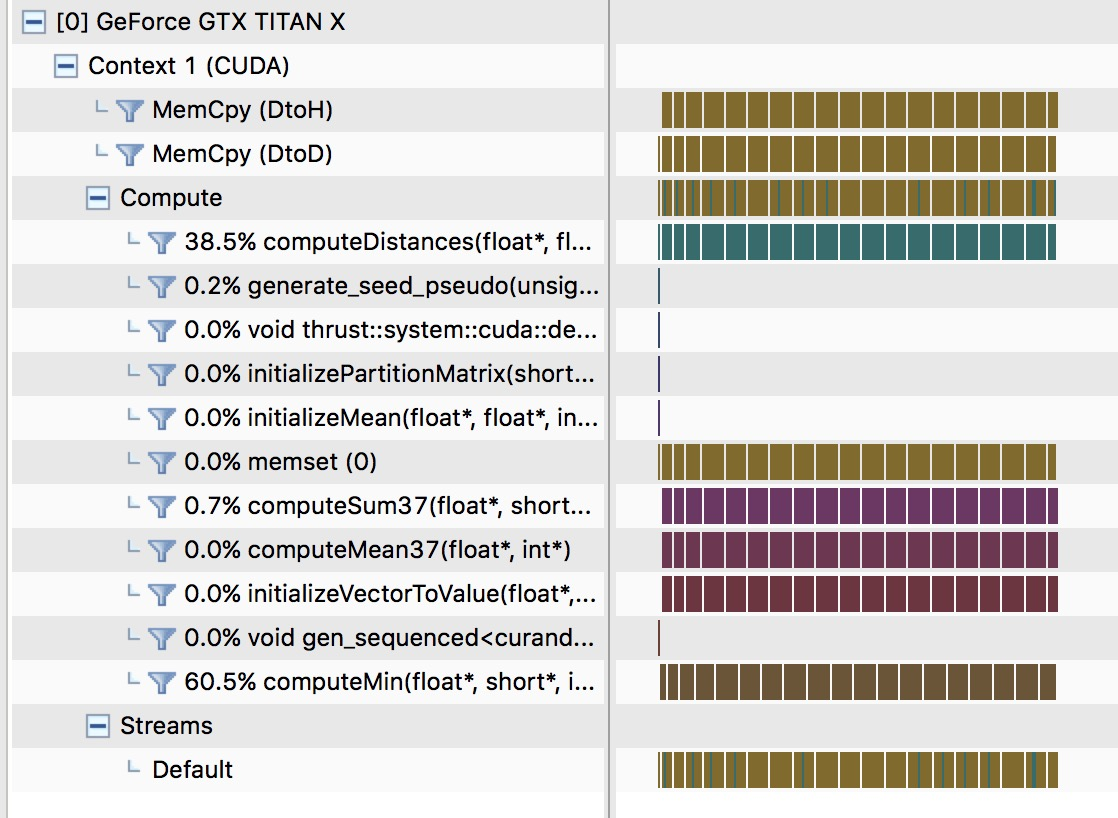
\includegraphics[width=\columnwidth]{Image/screen.jpg}
  \caption{Percentuale del tempo di esecuzione dei diversi kernel}
  \label{fig:screen}
\end{figure}


\begin{figure}[H]
  \centering
    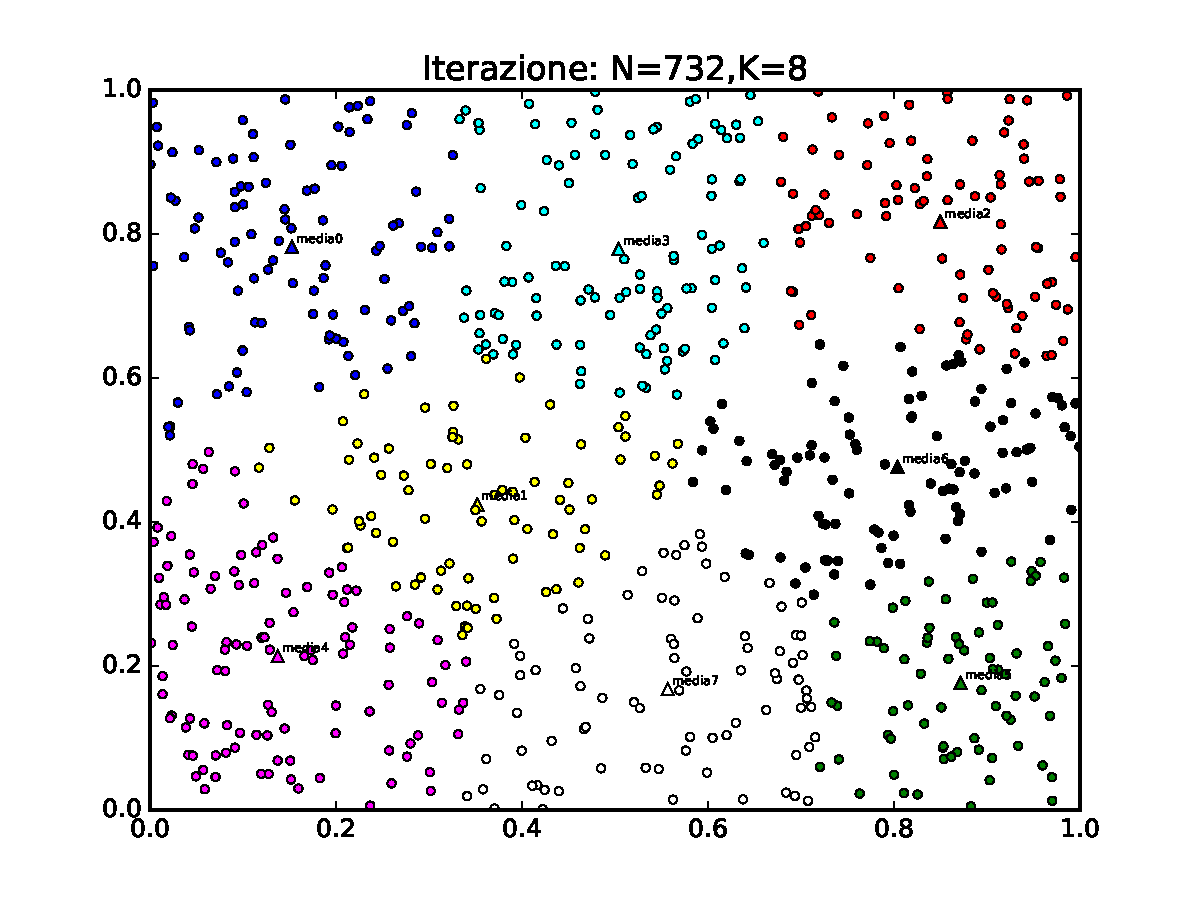
\includegraphics[width=\columnwidth]{Image/test.pdf}
  \caption{Plot per $N=732$ e $K=8$}
  \label{fig:test}
\end{figure}

\begin{figure}[H]
  \centering
    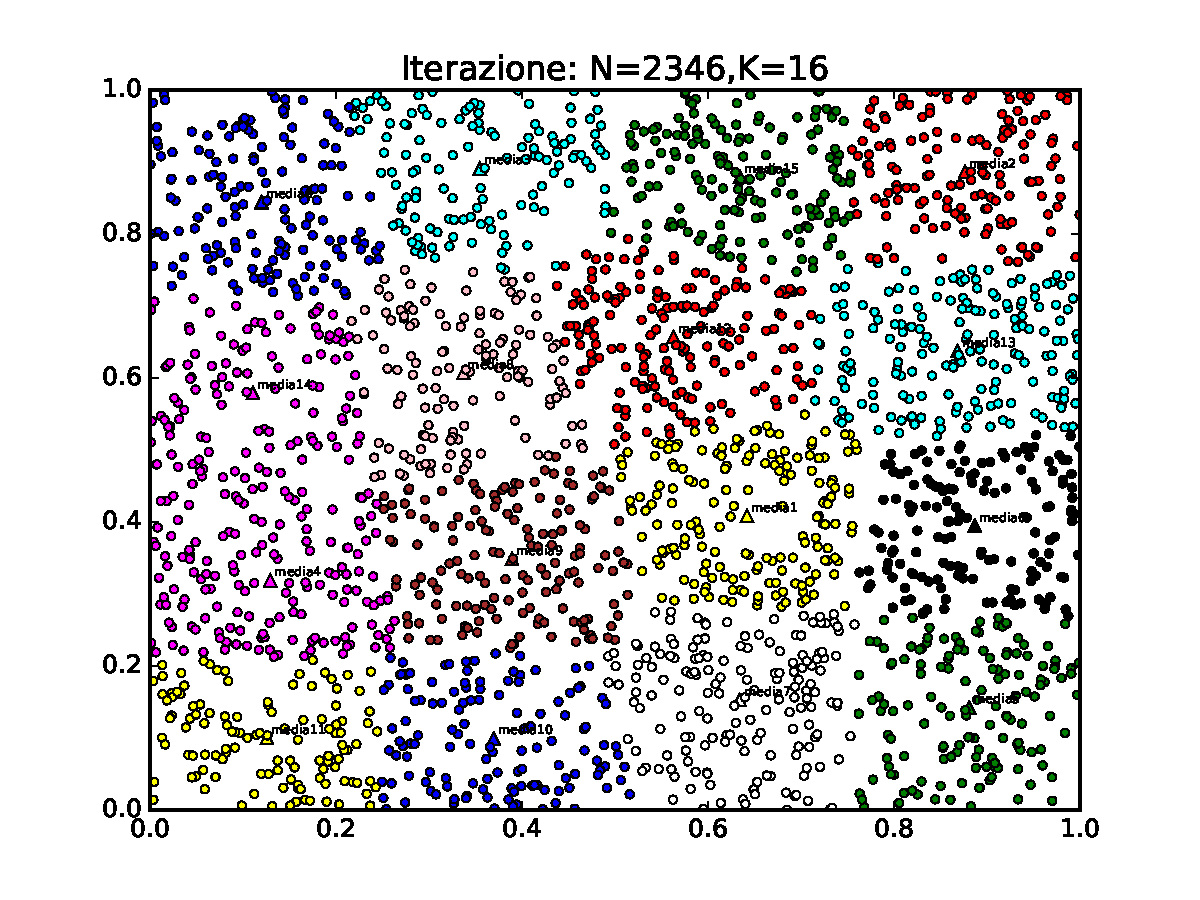
\includegraphics[width=\columnwidth]{Image/test2.pdf}
  \caption{Plot per $N=2346$ e $K=16$}
  \label{fig:test2}
\end{figure}

\begin{figure}[H]
  \centering
    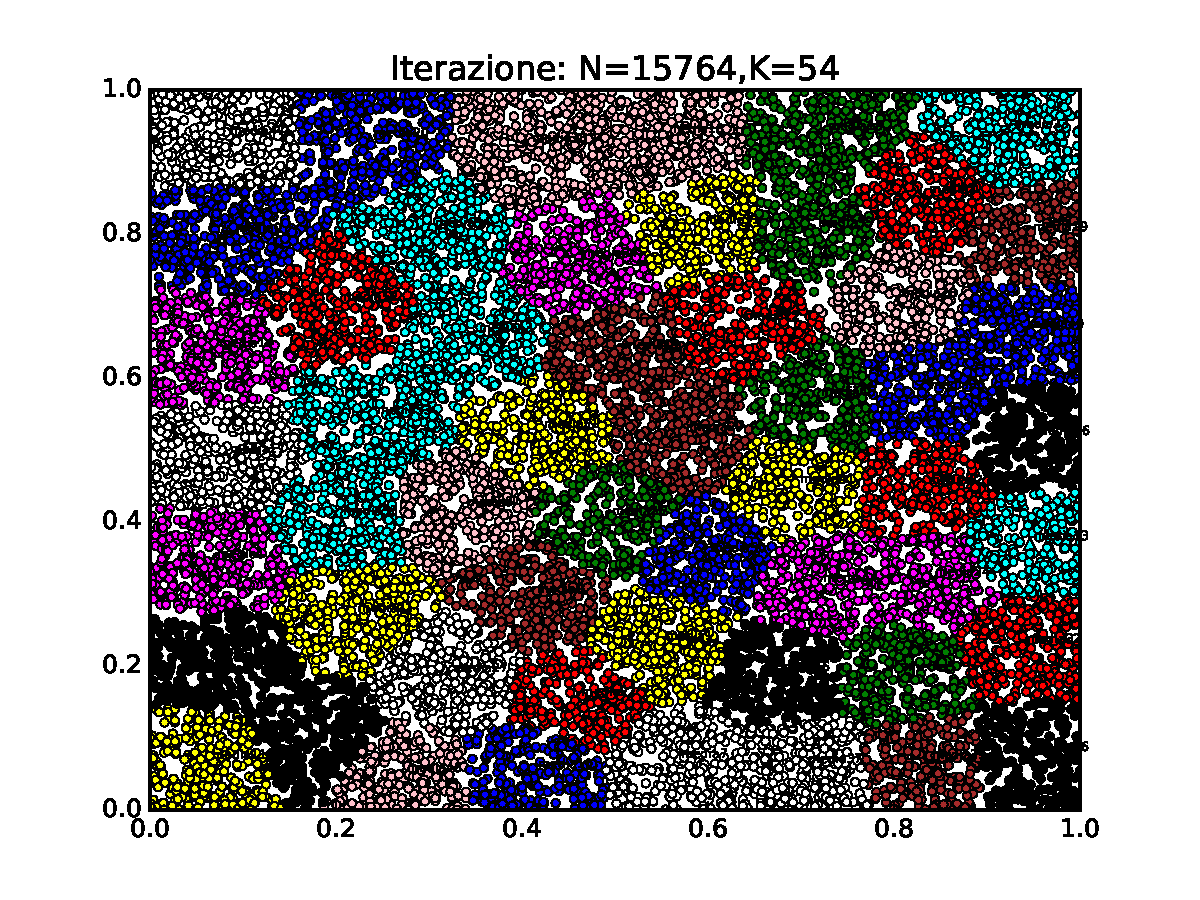
\includegraphics[width=\columnwidth]{Image/test3.pdf}
  \caption{Plot per $N=15764$ e $K=54$}
  \label{fig:test3}
\end{figure}


\section{Conclusioni}
È quindi possibile affermare che l'algoritmo di KMeans trae notevoli benefici da un'implementazione parallela che fa uso di una GPU. Infatti per gran parte dei calcoli è stato possibile realizzare una versione parallela in quanto indipendenti gli uni dagli altri. Alla luce degli esperimenti riportati non è possibile affermare che la percentuale di miglioramento della versione parallela rispetto alla sequenziale (speedup) sia legata alle due dimensioni principali del problema che sono state prese in considerazione, ovvero $N$ e $K$. Ad ogni modo la versione implementata in CUDA si è rivelata essere notevolmente più efficiente rispetto alla versione sequenziale sviluppata in C.
\vspace{3cm}

\appendix
\section{Codice}
\lstinputlisting[caption = Codice completo, style = customA, label = {code:completecode}]{Codice/KMeans.cu}
\bibliographystyle{plain}{}
\bibliography{bib.bib}




\end{document}
